%%%%%%%%%%%%%%%%%%%%%%%%%%%%%%%%%%%%%%%%%%%%%%%%%%%%%%%%%%%%%%%%%%%%%%%%%%%%%%%%
%% Plantilla de memoria en LaTeX para la ETSIT - Universidad Rey Juan Carlos
%%
%% Por Gregorio Robles <grex arroba gsyc.urjc.es>
%%     Grupo de Sistemas y Comunicaciones
%%     Escuela Técnica Superior de Ingenieros de Telecomunicación
%%     Universidad Rey Juan Carlos
%% (muchas ideas tomadas de Internet, colegas del GSyC, antiguos alumnos...
%%  etc. Muchas gracias a todos)
%%
%% La última versión de esta plantilla está siempre disponible en:
%%     https://github.com/gregoriorobles/plantilla-memoria
%%
%% Para obtener PDF, ejecuta en la shell:
%%   make
%% (las imágenes deben ir en PNG o JPG)

%%%%%%%%%%%%%%%%%%%%%%%%%%%%%%%%%%%%%%%%%%%%%%%%%%%%%%%%%%%%%%%%%%%%%%%%%%%%%%%%

\documentclass[a4paper, 12pt]{book}
%\usepackage[T1]{fontenc}

\usepackage[a4paper, left=2.5cm, right=2.5cm, top=3cm, bottom=3cm]{geometry}
\usepackage{times}
\usepackage[latin1]{inputenc}
\usepackage[spanish]{babel} % Comenta esta línea si tu memoria es en inglés
\usepackage{url}
%\usepackage[dvipdfm]{graphicx}
\usepackage{graphicx}
\usepackage{float}  %% H para posicionar figuras
\usepackage[nottoc, notlot, notlof, notindex]{tocbibind} %% Opciones de índice
\usepackage{latexsym}  %% Logo LaTeX

\title{Dr.Scratch Herramienta de análisis automático de proyectos Scratch}
\author{Cristian David Chushig Muzo}

\renewcommand{\baselinestretch}{1.5}  %% Interlineado

\begin{document}

\renewcommand{\refname}{Bibliografía}  %% Renombrando
\renewcommand{\appendixname}{Apéndice}

%%%%%%%%%%%%%%%%%%%%%%%%%%%%%%%%%%%%%%%%%%%%%%%%%%%%%%%%%%%%%%%%%%%%%%%%%%%%%%%%
% PORTADA

\begin{titlepage}
\begin{center}
\begin{tabular}[c]{c c}
%\includegraphics[bb=0 0 194 352, scale=0.25]{logo} &

\includegraphics[scale=0.25]{img/logo_vect.png} &
\begin{tabular}[b]{l}
\Huge
\textsf{UNIVERSIDAD} \\
\Huge
\textsf{REY JUAN CARLOS} \\
\end{tabular}
\\
\end{tabular}

\vspace{3cm}

\Large
INGENIER�A EN TELECOMUNICACIONES E INGENIER�A TÉCNICA EN SISTEMAS

\vspace{0.4cm}

\large
Curso Académico 2014/2015

\vspace{0.8cm}

Trabajo Fin de Carrera

\vspace{2.5cm}

\LARGE
Dr.Scratch Análisis automático de proyectos Scratch

\vspace{4cm}

\large
Autor : Cristian David Chushig Muzo \\
Tutor : Dr. Gregorio Robles \\
Co-Tutor: Jesús Moreno León
\end{center}
\end{titlepage}

\newpage
\mbox{}
\thispagestyle{empty} % para que no se numere esta pagina



%%%%%%%%%%%%%%%%%%%%%%%%%%%%%%%%%%%%%%%%%%%%%%%%%%%%%%%%%%%%%%%%%%%%%%%%%%%%%%%%
%%%% Para firmar
\clearpage
\pagenumbering{gobble}
\chapter*{}

\vspace{-4cm}
\begin{center}
\LARGE
\textbf{Proyecto Fin de Carrera}

\vspace{1cm}
\large
Dr.Scratch Herramienta de análisis automático de proyectos Scratch

\vspace{1cm}
\large
\textbf{Autor :} Cristian Chushig Muzo \\
\textbf{Tutor :} Dr. Gregorio Robles Martínez

\end{center}

\vspace{1cm}
La defensa del presente Proyecto Fin de Carrera se realizó el día \qquad$\;\,$ de \qquad\qquad\qquad\qquad \newline de 2015, siendo calificada por el siguiente tribunal:


\vspace{0.5cm}
\textbf{Presidente:}

\vspace{1.2cm}
\textbf{Secretario:}

\vspace{1.2cm}
\textbf{Vocal:}


\vspace{1.2cm}
y habiendo obtenido la siguiente calificación:

\vspace{1cm}
\textbf{Calificación:}


\vspace{1cm}
\begin{flushright}
Fuenlabrada, a \qquad$\;\,$ de \qquad\qquad\qquad\qquad de 2015
\end{flushright}



%%%%%%%%%%%%%%%%%%%%%%%%%%%%%%%%%%%%%%%%%%%%%%%%%%%%%%%%%%%%%%%%%%%%%%%%%%%%%%%%
%%%% Dedicatoria

\chapter*{}
\pagenumbering{Roman} % para comenzar la numeracion de paginas en numeros romanos
\begin{flushright}
\textit{Dedicado a \\
mi madre y su incansable  \\
esfuerzo de sacar adelante \\
a sus hijos}
\end{flushright}


%%%%%%%%%%%%%%%%%%%%%%%%%%%%%%%%%%%%%%%%%%%%%%%%%%%%%%%%%%%%%%%%%%%%%%%%%%%%%%%%
%%%% Agradecimientos

\chapter*{Agradecimientos}
%\addcontentsline{toc}{chapter}{Agradecimientos} % si queremos que aparezca en el índice
\markboth{AGRADECIMIENTOS}{AGRADECIMIENTOS} % encabezado

Ha sido muy duro el camino, pero sin duda ha valido la pena. Afrontar la aventura de
estudiar fuera de mi país natal es uno de mis mayores aciertos

El más grande de mis agradecimientos va dirigido a mi madre, aquella mujer luchadora que
con su esfuerzo ha sacado adelante a tres hijos. Ha sido un ejemplo de cómo se tiene que
conseguir lo que se quiere. Siempre llevo los valores inculcados, las costumbres dadas y
mi identidad en cada paso que doy, cualquier logro conseguido en mi vida se lo debo a ella.
Su pasión, su valor y su amor en todos estos años no sólo me han convertido en un profesional,
sino también en una persona de provechos. Un gracias nunca será suficiente, pero el
agradecimiento de corazón queda plasmado en estas pocas palabras.

También no quisiera olvidarme de mi familia en Quito, siempre han sido constantes los apoyos
recibidos y sin duda el cariño.

%%%%%%%%%%%%%%%%%%%%%%%%%%%%%%%%%%%%%%%%%%%%%%%%%%%%%%%%%%%%%%%%%%%%%%%%%%%%%%%%
%%%% Resumen

\chapter*{Resumen}
%\addcontentsline{toc}{chapter}{Resumen} % si queremos que aparezca en el índice
\markboth{RESUMEN}{RESUMEN} % encabezado


Este trabajo recoge el desarrollo de una plataforma web, Dr. Scratch, orientada a la 
evaluación de proyectos Scratch en relación a aspectos de pensamiento computacional. 
El núcleo de Dr. Scratch es \texttt{Hairball}, un framework usado para el análisis estático de 
proyectos Scratch a través de una consola Linux. Dr. Scratch presenta los resultados
de \texttt{Hairball} adaptados al público de la aplicación.

El objetivo principal es crear una herramienta automatizada y de fácil uso para el 
análisis de proyectos Scratch. Para esto, el interfaz usado es web y trata de ser 
lo más amigable posible con el público, especialmente niños y jóvenes que inician
su camino en el mundo de la programación.

El proyecto se ha realizado principalmente con el framework Django en la parte del
servidor, \texttt{Hairball} como núcleo y Bootstrap como framework para el \emph{front end}.

El proyecto Dr. Scratch se desarrolla dentro de una iniciativa del Grupo de Sistemas
y Comunicaciones (GSyC) de la Universidad Rey Juan Carlos (URJC) que investiga el
impacto del Desarrollo del pensamiento computacional y busca comprobar las destrezas
que se pueden potenciar en el contexto y proceso del aprendizaje de la programación.



%%%%%%%%%%%%%%%%%%%%%%%%%%%%%%%%%%%%%%%%%%%%%%%%%%%%%%%%%%%%%%%%%%%%%%%%%%%%%%%%
%%%% Resumen en inglés

\chapter*{Summary}
%\addcontentsline{toc}{chapter}{Summary} % si queremos que aparezca en el índice
\markboth{SUMMARY}{SUMMARY} % encabezado

Here comes a translation of the ``Resumen'' into English. Please, double check
it for correct grammar and spelling. As it is the translation of the ``Resumen'',
which is supposed to be written at the end, this as well should be filled out
just before submitting.


%%%%%%%%%%%%%%%%%%%%%%%%%%%%%%%%%%%%%%%%%%%%%%%%%%%%%%%%%%%%%%%%%%%%%%%%%%%%%%%%
%%%%%%%%%%%%%%%%%%%%%%%%%%%%%%%%%%%%%%%%%%%%%%%%%%%%%%%%%%%%%%%%%%%%%%%%%%%%%%%%
% Ã?NDICES %
%%%%%%%%%%%%%%%%%%%%%%%%%%%%%%%%%%%%%%%%%%%%%%%%%%%%%%%%%%%%%%%%%%%%%%%%%%%%%%%%

% Las buenas noticias es que los índices se generan automáticamente.
% Lo único que tienes que hacer es elegir cuáles quieren que se generen,
% y comentar/descomentar esa instrucción de LaTeX.

%%%% Ã?ndice de contenidos
\tableofcontents
%%%% Ã?ndice de figuras
\cleardoublepage
%\addcontentsline{toc}{chapter}{Lista de figuras} % para que aparezca en el indice de contenidos
\listoffigures % indice de figuras
%%%% Ã?ndice de tablas
%\cleardoublepage
%\addcontentsline{toc}{chapter}{Lista de tablas} % para que aparezca en el indice de contenidos
%\listoftables % indice de tablas


%%%%%%%%%%%%%%%%%%%%%%%%%%%%%%%%%%%%%%%%%%%%%%%%%%%%%%%%%%%%%%%%%%%%%%%%%%%%%%%%
%%%%%%%%%%%%%%%%%%%%%%%%%%%%%%%%%%%%%%%%%%%%%%%%%%%%%%%%%%%%%%%%%%%%%%%%%%%%%%%%
% INTRODUCCIÓN %
%%%%%%%%%%%%%%%%%%%%%%%%%%%%%%%%%%%%%%%%%%%%%%%%%%%%%%%%%%%%%%%%%%%%%%%%%%%%%%%%

\cleardoublepage
\chapter{Introducción}
\label{sec:intro} % etiqueta para poder referenciar luego en el texto con ~\ref{sec:intro}
\pagenumbering{arabic} % para empezar la numeración de página con números

El desarrollo de la tecnología está cambiando nuestros hábitos cotidianos: la forma
en que nos relacionamos con las personas, la manera de trabajar y significativamente
nuestra forma de aprender. El conocimiento ahora es global, al alcance de todos, con
una sencilla búsqueda a través de un dispositivo conectado a internet tenemos incontable
información en nuestras manos. Pero, girando la atención al uso de la tecnología en las 
aulas nos encontramos con un uso pasivo, convirtiendo al estudiante en usuario de 
aplicaciones. Los escolares, nativos digitales, conocen cómo buscar información en internet 
y manejar aplicaciones de una manera natural, pero la tecnología de trasfondo es invisible 
para ellos, lo que hace que pierdan muchas oportunidades y retos para su desarrollo en la
enseñanza de programación.
La programación en las aulas no es un descubrimiento nuevo, existen desde los años 60  con \texttt{Logo}. 
Pero, su popularidad se ha incrementando en los últimos años gracias a nuevas plataformas y aplicaciones
como \texttt{AppInventor}, \texttt{Stencyl}, \texttt{Alice}, \texttt{Etoys} y \texttt{Scratch}.

Y es Scratch donde gira el presente proyecto. Scratch ha tenido una penetración importante 
en la educación americana, y una de las muchas razones es su facilidad de aprendizaje. Los
bloques gráficos permiten a los usuarios un aprendizaje eficaz, y su entorno amigable permite 
la potenciación de la creatividad en el diseño y desarrollo de los proyectos.

El objetivo de la programación en edades tempranas es proveer de nuevas habilidades a niños y
jóvenes, habilidades necesarias en un entorno digital y globalizado. Encarar procesos de
autocorreción y búsqueda de errores, enfrentarse a retos de resolución de problemas son ejemplos
claros de éstas habilidades.







%%%%%%%%%%%%%%%%%%%%%%%%%%%%%%%%%%%%%%%%%%%%%%%%%%%%%%%%%%%%%%%%%%%%%%%%%%%%%%%%
%%%%%%%%%%%%%%%%%%%%%%%%%%%%%%%%%%%%%%%%%%%%%%%%%%%%%%%%%%%%%%%%%%%%%%%%%%%%%%%%
% OBJETIVOS %
%%%%%%%%%%%%%%%%%%%%%%%%%%%%%%%%%%%%%%%%%%%%%%%%%%%%%%%%%%%%%%%%%%%%%%%%%%%%%%%%

\cleardoublepage
\chapter{Objetivos}
\label{chap:objetivos}

\section{Objetivo general}
\label{sec:objetivo-general}

El objetivo general del proyecto es crear una herramienta y plataforma para que los
usuarios de Scratch puedan evaluar sus proyectos y hacer un seguimiento de su progreso
en relación a habilidades de pensamiento computacional.


\section{Objetivos específicos}
\label{sec:objetivos-especificos}

\begin{itemize}
  \item Crear una arquitectura software que permita la convergencia entre el framework \texttt{Hairball}
  con las tecnologías web, con el fin de mejorar su usabilidad y experiencia de usuario. En 
	primera instancia el análisis de los proyectos se hará subiéndolos en el formato sb2.
  \item Construir un modelo de datos que se adapte a la salida de datos que ofrece \texttt{Hairball} y
  parametrizarlo con las herramientas ofrecidas por Django.
  \item Adaptar el contexto ofrecido por Django a todo el potencial que ofrece Bootstrap como
  herramienta de \emph{front end}.
  \item Introducir técnicas de \emph{ludificación} dentro de la plataforma para atraer la atención y
  uso de los usuarios.
	\item Permitir un seguimiento de la evolución de los usuarios de Dr. Scratch en términos de 
	las habilidades de pensamiento computacional adquiridas a lo largo del uso de la plataforma
	mediante los proyectos evaluados.
\end{itemize}


%%%%%%%%%%%%%%%%%%%%%%%%%%%%%%%%%%%%%%%%%%%%%%%%%%%%%%%%%%%%%%%%%%%%%%%%%%%%%%%%
%%%%%%%%%%%%%%%%%%%%%%%%%%%%%%%%%%%%%%%%%%%%%%%%%%%%%%%%%%%%%%%%%%%%%%%%%%%%%%%%
% ESTADO DEL ARTE %
%%%%%%%%%%%%%%%%%%%%%%%%%%%%%%%%%%%%%%%%%%%%%%%%%%%%%%%%%%%%%%%%%%%%%%%%%%%%%%%%

\cleardoublepage
\chapter{Estado del arte}

En este capítulo se introducirán las bases tecnológicas más importantes del proyecto.


\section{Scratch}
\label{sec:seccion2}
Scratch es un proyecto del Grupo Lifelong Kindergarten del Laboratorio de Medios del MIT.
Scratch permite programar historias interactivas, juegos y animaciones a través de un
entorno completamente visual. Se fundamenta en el uso de personajes, escenarios y bloques
gráficos con una funcionalidad específica que permite crear una lógica e interacción
entre los elementos. Además Scratch es gratuito, de uso libre, multilenguaje y es muy
recomendado para la iniciación en el mundo de la programación. Su uso se ha intensificado
en los últimos años y dentro de su nube tiene millones de proyectos almacenados que
pueden ser compartidos y vistos por otros usuarios Scratch.


\section{\texttt{Hairball}}
\label{sec:seccion3}
\texttt{Hairball} es un framework utilizado para el análisis de proyectos Scratch. Creado por Bryce
Boe en la universidad de Santa Barbara. \texttt{Hairball} se constituye esencialmente de plugins.
Los plugins iniciales fueron desarrollados por la universidad de Santa Barbara, y a estos se
suman otros plugins programados por la universidad Rey Juan Carlos y en concreto por Jesús Moreno Léon.
El framework es de libre acceso y está disponible en la red.\footnote{\url{http://github.com/ucsb-cs-education/Hairball}}.

Los plugins que se puedan encontrar en la última versión de \texttt{Hairball} son:

\begin{itemize}
  \item \texttt{blocks.DeadCode}.
  Busca código que no llega a ejecutarse nunca, parametrizándolo en un valor entero.
  \item \texttt{blocks.BlockCounts}.
  Cuenta el número de bloques asociados al proyecto y devuelve su valor en un entero.
  \item \texttt{initialization.AttributeInitialization}.
  Busca propiedades de los personajes que son modificadas en algún punto del programa,
  pero que no se inicializan al comenzar la 	ejecución del proyecto. Por cada propiedad
  analizada del personaje: posición, tamaño, 	disfraz, visibilidad y orientación, se
  muestra un valor 0 si la propiedad no se modifica, 	1 si se modifica pero no se inicializa,
  2 si se inicializa correctamente.
  \item \texttt{duplicate.DuplicateScripts}.
  Busca programas repetidos en el proyecto. Programas que deberían haber sido implementados
  con un método definido por el programador.
  \item \texttt{mastery.Mastery}.
  Asigna una puntuación que indica el grado de maestría demostrado en la programación del
  proyecto para diferentes aspectos: abstracción, paralelización, razonamiento lógico,
  sincronización, control de flujo, interactividad con el usuario, representación de la información.
	
	
\end{itemize}


\section{Django}
\label{sec:seccion4}
Django es un framework web de código abierto escrito en \texttt{Python} que permite construir aplicaciones
web más rápido y con menos código. Proporciona un conjunto de herramientas para crear aplicaciones
siguiendo los principios de \texttt{DRY} (\emph{Don't Repeat Yourself}), para evitar la duplicidad de líneas de código.
Se basa en el diseño \texttt{MVC} (Modelo Vista Controlador), lo que le brinda independencia y permite que
las partes funcionales estén claramente separadas.
Django permite la conexión con distintos sistemas de bases de datos como MySQL, Oracle.



\section{Bootstrap}
\label{sec:seccion5}
Bootstrap es un framework desarrollado por Twitter para crear interfaces y diseños web responsive
basados en HTML5 y CSS3. Su principal ventaja es la de adaptar la interfaz de la aplicación web
al tamaño del dispositivo desde donde se está accediendo. La documentación ofrecida permite la
construcción de webs de forma eficaz.






%%%%%%%%%%%%%%%%%%%%%%%%%%%%%%%%%%%%%%%%%%%%%%%%%%%%%%%%%%%%%%%%%%%%%%%%%%%%%%%%
%%%%%%%%%%%%%%%%%%%%%%%%%%%%%%%%%%%%%%%%%%%%%%%%%%%%%%%%%%%%%%%%%%%%%%%%%%%%%%%%
% DISEÑO E IMPLEMENTACIÓN %
%%%%%%%%%%%%%%%%%%%%%%%%%%%%%%%%%%%%%%%%%%%%%%%%%%%%%%%%%%%%%%%%%%%%%%%%%%%%%%%%

\cleardoublepage
\chapter{Diseño e implementación}

Este capítulo es el eje principal del proyecto, en el que se describe la arquitectura,
el diseño y se hace una descripción de las funcionalidades más importantes de Dr.
Scratch. Está dividido en tres partes: el servidor basado en Django, el framework
\texttt{Hairball} y el frontEnd basado en Bootstrap.

\section{Arquitectura general}
\label{sec:arquitectura}

La arquitectura de Dr. Scratch se muestra en la figura 4.1. Está claramente identificado
con el modelo cliente-servidor. El usuario a través de un navegador subirá su proyecto
o introducirá el identificador a través de un formulario. Esta petición será recogida 
por el manejador de Django será procesada por un método asociada a la URL, dentro de 
este método se llamará a los plugins de \texttt{Hairball} recogiendo los datos parametrizados en
el modelo de datos para su almacenamiento, y se responderá renderizando el contenido
en un template.

\begin{itemize}
  \item Servidor. Se basa principalmente en Django. Django permite la abstracción de la
	base de datos, el modelo vista controlador y la interacción con el componente \emph{front end}.
  \item \texttt{Hairball}. Es un framework que permite el análisis de proyectos Scratch. Su uso es
	a través de una consola \texttt{bash}. \texttt{Hairball} se compone de plugins, para usar cada uno se
	tiene que realizar una llamada independiente por consola.
  \item Cliente. Generalmente el acceso a la plataforma se hace mediante un navegador. El
	desarrollo de la parte \emph{front end} se realiza conjuntamente con Django y Bootstrap, este
	último permite una funcionalidad \emph{responsive} lo que permite que el acceso a Dr. Scratch
	puede hacerse por un dispositivo móvil o tablet, sin la pérdida del diseño original.
	
\end{itemize}


\section{Diseño e implementación del servidor}
\label{sec:servidor}

El diseño e implementación del servidor se basa en dos partes representativas. Por un lado todo lo
correspondiente a la plataforma web con Django y por otro la incorporación de la funcionalidad de
\texttt{Hairball} y su correspondiente tratamiento de información.

\subsection{Conexión con \texttt{Hairball}}

\texttt{Hairball} provee la salida de datos a través de la consola. Para cada plugin de \texttt{Hairball} se debe hacer una llamada
a través de la consola. En esta sección se detalla con ejemplos las salidas de cada uno de los plugins usados en
Dr.Scratch, ya que esto contribuirá al entendimiento del modelo de datos del proyecto.

Cada uno de los plugins se ejecutan a través de una consola \texttt{bash} y su modo de uso es el siguiente:

\begin{center}
\texttt{Hairball} -p "`plugin-\texttt{Hairball}"' "`nombre-proyecto-formato-sb2"'
\end{center}

Para evaluar las salidas de \texttt{Hairball} se usará el proyecto Scratch test-project.sb2, descargado a través de la 
nube de Scratch.\footnote{\url{scratch.mit.edu/}}

Para usar el plugin DeadCode se hace la siguiente llamada.
\begingroup
\fontsize{7pt}{8pt}\selectfont
\begin{verbatim}
$ \texttt{Hairball} -p blocks.DeadCode test-project.sb2 
test-project.sb2 
'Stage': [kurt.Script([ 
    kurt.Block('whenIReceive', u'never'), 
    kurt.Block('startScene', u'castle')], pos=(366, 155)), 
           kurt.Script([  
    kurt.Block('whenIReceive', u'yeppers'), 
    kurt.Block('startScene', u'castle')], pos=(229, 243)), 
           kurt.Script([ 
    kurt.Block('whenIReceive', u'no'), 
    kurt.Block('startScene', u'castle')], pos=(85, 312))] 
\end{verbatim}
\endgroup


De la salida se deduce que para el proyecto Scratch test-project.sb2 existen 6 bloques de código muerto dentro de 3 scripts. Además se puede tener la información de la posición asociado al código muerto.

Para el uso del plugin AttributeInitialization se presenta la siguiente salida:

\begingroup
\fontsize{7pt}{8pt}\selectfont
\begin{verbatim}
$ \texttt{Hairball} -p initialization.AttributeInitialization test-project.sb2 
test-project.sb2
{u'frozen_elsa_by_meddek-d6w674h': {'position': 2, 'size': 0, 'costume': 0, 'visibility': 2, 'orientation': 0}, 
u'Sprite8': {'position': 0, 'size': 0, 'costume': 0, 'visibility': 2, 'orientation': 0}, 
u'ElsaPose': {'position': 2, 'size': 0, 'costume': 0, 'visibility': 2, 'orientation': 0}, 
u'Sprite4': {'position': 2, 'size': 0, 'costume': 0, 'visibility': 2, 'orientation': 0}, 
'stage': {'background': 2}, 
u'Sprite2': {'position': 0, 'size': 0, 'costume': 0, 'visibility': 2, 'orientation': 0},
 u'Sprite3': {'position': 2, 'size': 0, 'costume': 1, 'visibility': 2, 'orientation': 0},
 u'Sprite1': {'position': 2, 'size': 0, 'costume': 0, 'visibility': 2, 'orientation': 0}}
\end{verbatim}
\endgroup

Este plugin busca propiedades de los personajes que son modificadas en algún punto del 
proyecto, pero que no se inicializaron al comenzar el flujo del programa. Las propiedades 
de los personajes son: position, size, costume, visibility, orientation. Por cada propiedad
analizada de cada personaje se muestra un valor parametrizado: un 0 si no ha modificado, un
1 si se modifica pero no se inicializa, 2 si se inicializa correctamente. Por lo tanto, las
propiedades que tienen un valor de 1 tienen un error de programación, y serán las propiedades
que tienen el valor 1 las que se almacenan para su posterior tratamiento.


Para el uso del plugin Sprite naming se presenta la siguiente salida:

\begingroup
\fontsize{7pt}{8pt}\selectfont
\begin{verbatim}
$ \texttt{Hairball} -p convention.SpriteNaming test-project.sb2 
test-project.sb2
5 default sprite names found:
Sprite2
Sprite8
Sprite1
Sprite4
Sprite3
\end{verbatim}
\endgroup

Este plugin busca los personajes del proyecto que han mantenido el nombre por defecto. En
la salida se puede observar un listado de los nombres de esto personajes. Lo que se 
almacenará dentro de la base de datos será el nombre por defecto que aparece en el listado
de la salida del plugin. En el ejemplo anterior: Sprite2, Sprite8, Sprite1, Sprite4, Sprite3.

Para el uso del plugin DuplicateScripts se muestra la siguiente salida:
$ \texttt{Hairball} -p duplicate.DuplicateScripts test-project.sb2 
test-project.sb2
4 duplicate scripts found
['when @greenFlag clicked', 'set rotation style %s', 'forever%s', 'move %s steps', 'if on edge, bounce']
['when @greenFlag clicked', 'set rotation style %s', 'forever%s', 'move %s steps', 'if on edge, bounce']
['when @greenFlag clicked', 'forever%s', 'next costume', 'wait %s secs']
['when @greenFlag clicked', 'forever%s', 'if %s then%s', 'say %s for %s secs', 'stop %s', 'touching %s?']
\end{verbatim}
\endgroup


Por último, se detalla el plugin que ofrece resultados cuantificables del pensamiento 
computacional, y es el más importante desde el punto de vista de información relevante
al usuario, el plugin Mastery.


\begingroup
\fontsize{7pt}{8pt}\selectfont
\begin{verbatim}
$ \texttt{Hairball} -p mastery.Mastery test-project.sb2 
test-project.sb2
{'Abstraction': 2, 'Parallelization': 1, 'Logic': 1, 'Synchronization': 2, 'FlowControl': 2, 'UserInteractivity': 2, 'DataRepresentation': 2}
Total mastery points: 12/21
Average mastery points: 1.71/3
Overall programming competence: Developing
\end{verbatim}
\endgroup

Este plugin no tiene presente los errores encontrados en los otros plugins mencionados.
Analiza el proyecto Scratch y asigna una puntuación que cuantifica el grado de expertise
mostrado en la programación para diferentes aspectos del pensamiento computacional: la
abtracción, paralelización, razonamiento lógico, sincronización, control de flujo,
interactividad con el usuario y representación de la información. Cada aspecto tiene
una puntuación máxima de 3, siendo 1 el nivel más básico y 3 un nivel más experto. En
total la suma de los 7 aspectos es 21. El plugin suma los valores obtenidos en cada 
aspecto del pensamiento computacional y en función del resultado sacado asigna un
nivel de maestría para el proyecto analizado, siendo los niveles: básico, en desarrollo
y profesional.


\subsection{Modelo de datos}
El modelo de datos tiene como objetivo adecuarse a las salidas de consola de \texttt{Hairball}. Una de las principales ventajas de Django es que la conexión con los sistemas de bases de datos es transparente para el usuario. 
Simplemente se debe realizar la respectiva configuración en el fichero settings.py de la base de datos. Para este proyecto se uso en primera instancia SQlite.

Para la especificación del modelo de datos en Django se debe modificar el fichero models.py. 


\begin{figure}
  \centering
  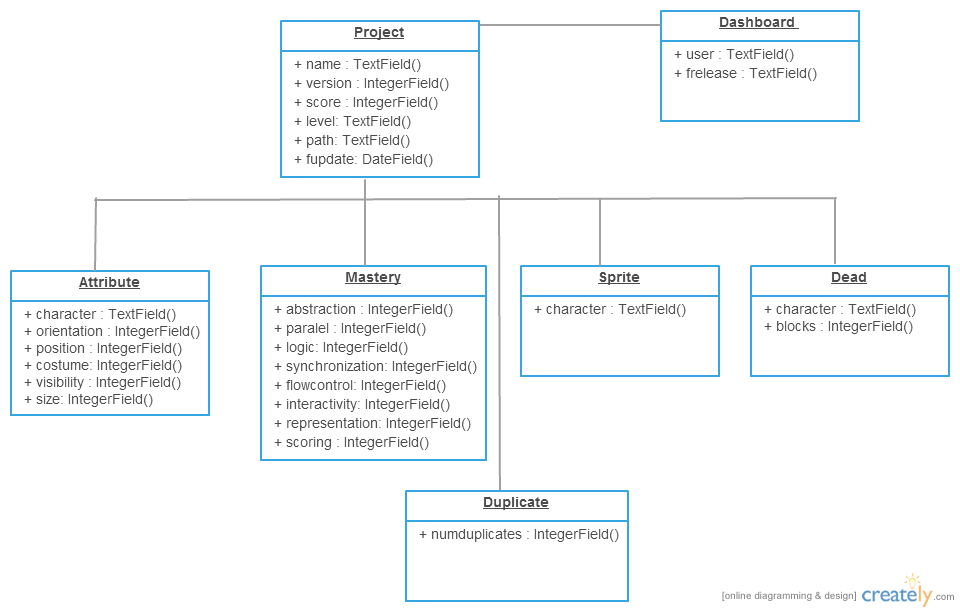
\includegraphics{img/modelo}
  \caption{Estructura del parser básico}
\end{figure}


\section{Diseño e implementación del cliente}
\label{sec:cliente}

El modelo de datos se construye de acuerdo a las salidas de datos ofrecidas por los plugins de
\texttt{Hairball}.




%%%%%%%%%%%%%%%%%%%%%%%%%%%%%%%%%%%%%%%%%%%%%%%%%%%%%%%%%%%%%%%%%%%%%%%%%%%%%%%%
%%%%%%%%%%%%%%%%%%%%%%%%%%%%%%%%%%%%%%%%%%%%%%%%%%%%%%%%%%%%%%%%%%%%%%%%%%%%%%%%
% RESULTADOS %
%%%%%%%%%%%%%%%%%%%%%%%%%%%%%%%%%%%%%%%%%%%%%%%%%%%%%%%%%%%%%%%%%%%%%%%%%%%%%%%%

\cleardoublepage
\chapter{Resultados}


%%%%%%%%%%%%%%%%%%%%%%%%%%%%%%%%%%%%%%%%%%%%%%%%%%%%%%%%%%%%%%%%%%%%%%%%%%%%%%%%
%%%%%%%%%%%%%%%%%%%%%%%%%%%%%%%%%%%%%%%%%%%%%%%%%%%%%%%%%%%%%%%%%%%%%%%%%%%%%%%%
% CONCLUSIONES %
%%%%%%%%%%%%%%%%%%%%%%%%%%%%%%%%%%%%%%%%%%%%%%%%%%%%%%%%%%%%%%%%%%%%%%%%%%%%%%%%

\cleardoublepage
\chapter{Conclusiones}
\label{chap:conclusiones}


\section{Consecución de objetivos}
\label{sec:consecucion-objetivos}

El presente proyecto consiguió el objetivo general que se planteó, la 
construcción de una plataforma web donde los usuarios de Scratch pueden 
obtener una valoración de sus proyectos. Esta plataforma es una versión
beta de Dr. Scratch, las nuevas funcionalidades y el potencial de Dr. 
Scratch da un espectro de desarrollo importante y atractivo.

Dentro de los objetivos específicos también se puede valorar de manera
positiva toda la labor de desarrollo. La convergencia del framework
\texttt{Hairball} con Django fue satisfactorio. Se logró parametrizar las salidas
que ofrecía cada plugin de \texttt{Hairball} dentro de un contexto de modelo de
datos, y gracias a esto tener una estructura fiable para el almacenamiento
y extracción de los componentes de pensamiento computacional asociados
a cada proyecto. En las primeras versiones del modelo de datos se notó
las posibles mejoras para hacer más consistente las relaciones entre las
distintas tablas y se optó por la reformulación del modelo de datos hasta
que se obtuvo una versión que a nuestro parecer era viable y era capaz
de soportar las consultas realizadas por el componente \emph{front end} de una
manera eficiente, sin repercutir en términos de rendimiento.

Uno de los aportes no contemplados en los objetivos iniciales fue la
manera en cómo el usuario mete su proyecto dentro de la plataforma
para analizarlo. En primera instancia se decidió subirlo a Dr. Scratch
para evaluarlo, pero se comprobó que la eficiencia no era del todo
buena, así que se cambió el enfoque y haciendo uso de la API de Scratch
y del aporte de un script hecho por un desarrollador externo se 
obtuvo otro método más eficaz. Simplemente con la introducción del 
identificador del proyecto que se asocia en la nube de Scratch ahora
se puede realizar el análisis, todo esto repercutiendo en la optimización 
de respuesta del servidor al usuario.


En el objetivo de introducir ludificación dentro de Dr. Scratch la 
valoración no fue satisfactoria. Pese a que hubo contactos con las 
técnicas de ludificación, éstas no fueron incluidas principalmente 
por términos de tiempo y focalización en otras funcionalidades que 
se consideraban con un grado mayor de relevancia. Una de las medidas
adoptadas para la inclusión de la ludificación dentro de Dr. Scratch
fue elaborar funciones y procedimientos de almacenamiento de la 
información más óptimos. Las versiones iniciales de los métodos para 
almacenar los datos importantes de los plugins no eran demasiado 
óptimos en relación a la modularidad. Así pues, en la última versión
de los procs usados se optó por dar independencia entre los datos de 
los plugins, así como reformular varios campos de las tablas del
modelo de datos, el resultado fue una robustez y optimización en la
adquisición de datos que para una versión futura de Dr. Scratch 
permitirá una mayor integración con la ludificación, ya que el 
tratamiento de los datos será importante.

Otro de los hitos que no se pudo cumplir fue la construcción de una
funcionalidad que permita el seguimiento de los usuarios para poder
evaluar su progreso en el grado de adquisición de habilidades de 
pensamiento computacional. Se hizo un seguimiento e hincapié en la 
introducción de este componente, pero también por motivos de tiempo
no fue posible su integración. 


\section{Aplicación de lo aprendido}
\label{sec:aplicacion}

Sin lugar a dudas los conocimientos aprendidos en la asignatura de Servicios
y Aplicaciones Telemáticas (SAT) han sido vitales para el desarrollo del 
proyecto. Todas las nociones básicas del desarrollo web, cómo se procesan
las peticiones HTTP, la iniciación en HTML y CSS para la parte Front End.
En SAT también aprendí a usar Django, la parte núcleo con la que se 
desarrolla el servidor de Dr. Scratch. Tuve contanto con el concepto de 
modelo vista y controlador, que es el paradigma que usa Django. El modo
en cómo crear una aplicación RESTful a través de las funcionalidades de

Además, debo mencionar otros conocimientos adquiridos por asignaturas como
Diseño de Bases de Datos, Metodología de la programación y Estructura de 
Datos me han permitido tener una visión más global y abstracta a la hora
de establecer la lógica y flujo del programa.



\section{Lecciones aprendidas}
\label{sec:lecciones_aprendidas}

La lección más importante es como trabajar con distintas tecnologías para
conseguir un objetivo común. El hecho de juntar diversos frameworks era
un reto, ya que se debían establecer las pautas para su comunicación y 
que esta sea fiable y eficaz. En un principio, el mayor reto estaba en el
framwork Hairball, que era un poco desconocido, pero se logró salir con
resultados positivos.

Otro de los puntos positivos fue aprendar de diseño y maquetación web. Dentro
de la carrera aprendimos como usar Django para desarrollar el servidor, 
procesar las peticiones y la inclusión de templates, pero esto centrándonos
en mayor medida en la parte de lógica, sin meternos demasiado en la parte
de Front End. Con esto proyecto aprendí a usar Bootstrap y darle un matiz
más profesional a mis aplicaciones web, además de poder crear aplicaciones
responsive que puedan ser abiertas sin pérdida de estilo en cualquier
dispositivo móvil. 

Por último quisiera señalar un aspecto que nuevo y novedoso que me aportó
gran interés, el pensamiento computacional. La introducción de la 
programación dentro de la enseñanza de los niños con el fin de adquirir
nuevas habilidades muy útiles dentro del contexto actual. Descubrí que 
la programación ayuda y tiene un impacto enorme en como evolucionan 
ciertas partes de nuestro cerebro, y aunque de estos matices todavía
no he profundizado, sin duda es un área que me incentiva a continuar con
una investigación.


\section{Trabajos futuros}
\label{sec:trabajos_futuros}


Sin lugar a dudas Dr. Scratch tiene muchas funcionalidades que puede ser agregadas
y muchas otras que pueden ser optimizadas.


\begin{enumerate}
  \item Componente de red social. La interacción entre usuarios de Dr. Scratch y su
	cooperación es sin duda un punto fuerte de mejora para la plataforma. La posibilidad
	de que los usuarios puedan competir por mejorar sus habilidades de pensamiento
	computacional requerirá nuevas herramientas dentro de Dr. Scratch, por ejemplo, la
	inclusión de comentarios, poder dar validaciones entre usuarios de las habilidades
	adquiridas o poder conectar Dr. Scratch con redes sociales son sólo pequeños ejemplos.
  \item Creación de APIs. La posibilidad de que Dr. Scratch puede interactuar con
	otros sistemas o aplicaciones puede ser muy novedoso. Para ello, la implementación
	de APIs que tengan la capacidad de establecer comunicaciones de manera coherente y
	sin pérdida de seguridad es vital. Además, las APIs no sólo servirían a otras
	plataformas, también permitirán que usuarios con un conocimiento más experto pueda
	hacer uso de estas librerías para automatizar tareas de análisis de proyectos 
	reduciendo considerablemente los tiempos.
	\item Peticiones asíncronas. En este punto, Dr. Scratch es capaz de resolver las
	peticiones de usuarios sin problemas, pero toda su funcionamiento se hace de una
	manera muy estática, refiriéndome a cómo se procesan las peticiones y se responden
	a estas. Otra línea de mejora es darle un contexto asíncrono, que todas las 
	peticiones de análisis se hagan por AJAX por ejemplo.
	\item Seguridad. Pese a que el proyecto se desarrolló con frameworks y tecnología 
	muy fiable y probada por muchos usuarios, existe una línea de mejora que es 
	significativa, la seguridad. Una revisión y una planificación de validaciones del
	software podría evitar vulnerabilidades que se nos escapa en este punto. 
\end{enumerate}







%%%%%%%%%%%%%%%%%%%%%%%%%%%%%%%%%%%%%%%%%%%%%%%%%%%%%%%%%%%%%%%%%%%%%%%%%%%%%%%%
%%%%%%%%%%%%%%%%%%%%%%%%%%%%%%%%%%%%%%%%%%%%%%%%%%%%%%%%%%%%%%%%%%%%%%%%%%%%%%%%
% APÉNDICE(S) %
%%%%%%%%%%%%%%%%%%%%%%%%%%%%%%%%%%%%%%%%%%%%%%%%%%%%%%%%%%%%%%%%%%%%%%%%%%%%%%%%

\cleardoublepage
\appendix
\chapter{Instalación y uso de \texttt{Hairball}}
\label{app:manual}




%%%%%%%%%%%%%%%%%%%%%%%%%%%%%%%%%%%%%%%%%%%%%%%%%%%%%%%%%%%%%%%%%%%%%%%%%%%%%%%%
%%%%%%%%%%%%%%%%%%%%%%%%%%%%%%%%%%%%%%%%%%%%%%%%%%%%%%%%%%%%%%%%%%%%%%%%%%%%%%%%
% BIBLIOGRAFIA %
%%%%%%%%%%%%%%%%%%%%%%%%%%%%%%%%%%%%%%%%%%%%%%%%%%%%%%%%%%%%%%%%%%%%%%%%%%%%%%%%

\cleardoublepage


\end{document}
